\newpage
\section{THEORETICAL PART}

%%%%%%%%%%%%%%%%%%%%%%%%%%%%%%%%%%%%%%%%%%%%%%%%%%%%%%%%%%%%%%%%%%%%%%%%%%%%%%%%%%%%%%%%
%%%%%%%%%%%%%%%%%%%%%%%%%%%%%%%%%%%%%%%%%%%%%%%%%%%%%%%%%%%%%%%%%%%%%%%%%%%%%%%%%%%%%%%%
In order to convert a real system consisting of individual molecules into a form that can be understood by a computer software, we must define individual parameters that are essential for describing mutual interactions of atoms. When describing real systems, it is usually necessary to consider a certain degree of approximation due to the possible computational complexity. In computational chemistry methods, we often encounter the so-called Born-Oppenheimer approximation, which is based on the decoupling of the motion of nuclei and electrons. The basis of the approximation is the orders-of-magnitude difference in mass between the electron and the nucleus. The latter thus move very slowly relative to the electrons and can thus be considered as a fixed point charge. This allows us to calculate the energy of a molecule as a function of the positions of the nuclei, in quantum chemistry we talk about the so-called Potential Energy Surface (PES), which is a function of 3$N$ coordinates, where $N$ is the number of nuclei. \cite{leach_molecular_2001} 

For small systems, it is possible to calculate the PES based on quantum chemistry methods using reasonable resources, for very large systems this is not yet realistic. We therefore introduce a classical-mechanics set of analytic functions, yet empiric parameters called the Force Field (FF), which enable to evaluate the energy of simulated systems depending on the positions of the nuclei. Methods based on the use of such Force Fields are called molecular mechanics, which are applied especially when quantum phenomena are not of great importance and we can use classical mechanics approach or big amorphous systems where quantum-based calculations would be extremely expensive and resource taking. \cite{monticelli_force_2013}

\subsection{Force fields}
The total energy calculated using the force field can be broken down into two contributions, a binding and a non-binding term, which are further expanded in Equations \ref{eq:ff2} and \ref{eq:ff3}.

\begin{comment}
	\begin{equation}\label{eq:ff1}
		E_{\text{total}} = E_{\text{bonded}} + E_{\text{nonbonded}}
	\end{equation}.
\end{comment}


\begin{equation}\label{eq:ff2}
	E_{\text{bonded}} = E_{\text{bond}} + E_{\text{angle}} + E_{\text{torsion}}
\end{equation}

\begin{equation}\label{eq:ff3}
	E_{\text{nonbonded}} = E_{\text{electrostatic}} + E_{\text{Van der Walls}}
\end{equation}

%To get a better idea of what lies behind the individual terms, visualization of the corresponding mechanistic degrees of freedom is in the Figure \ref{fig:ff}. OBRÁZEK VYTVOŘÍM VLASTNÍ V PODOBNÉM DUCHU----
%
%\begin{figure}[htb!]
%	\centering
%	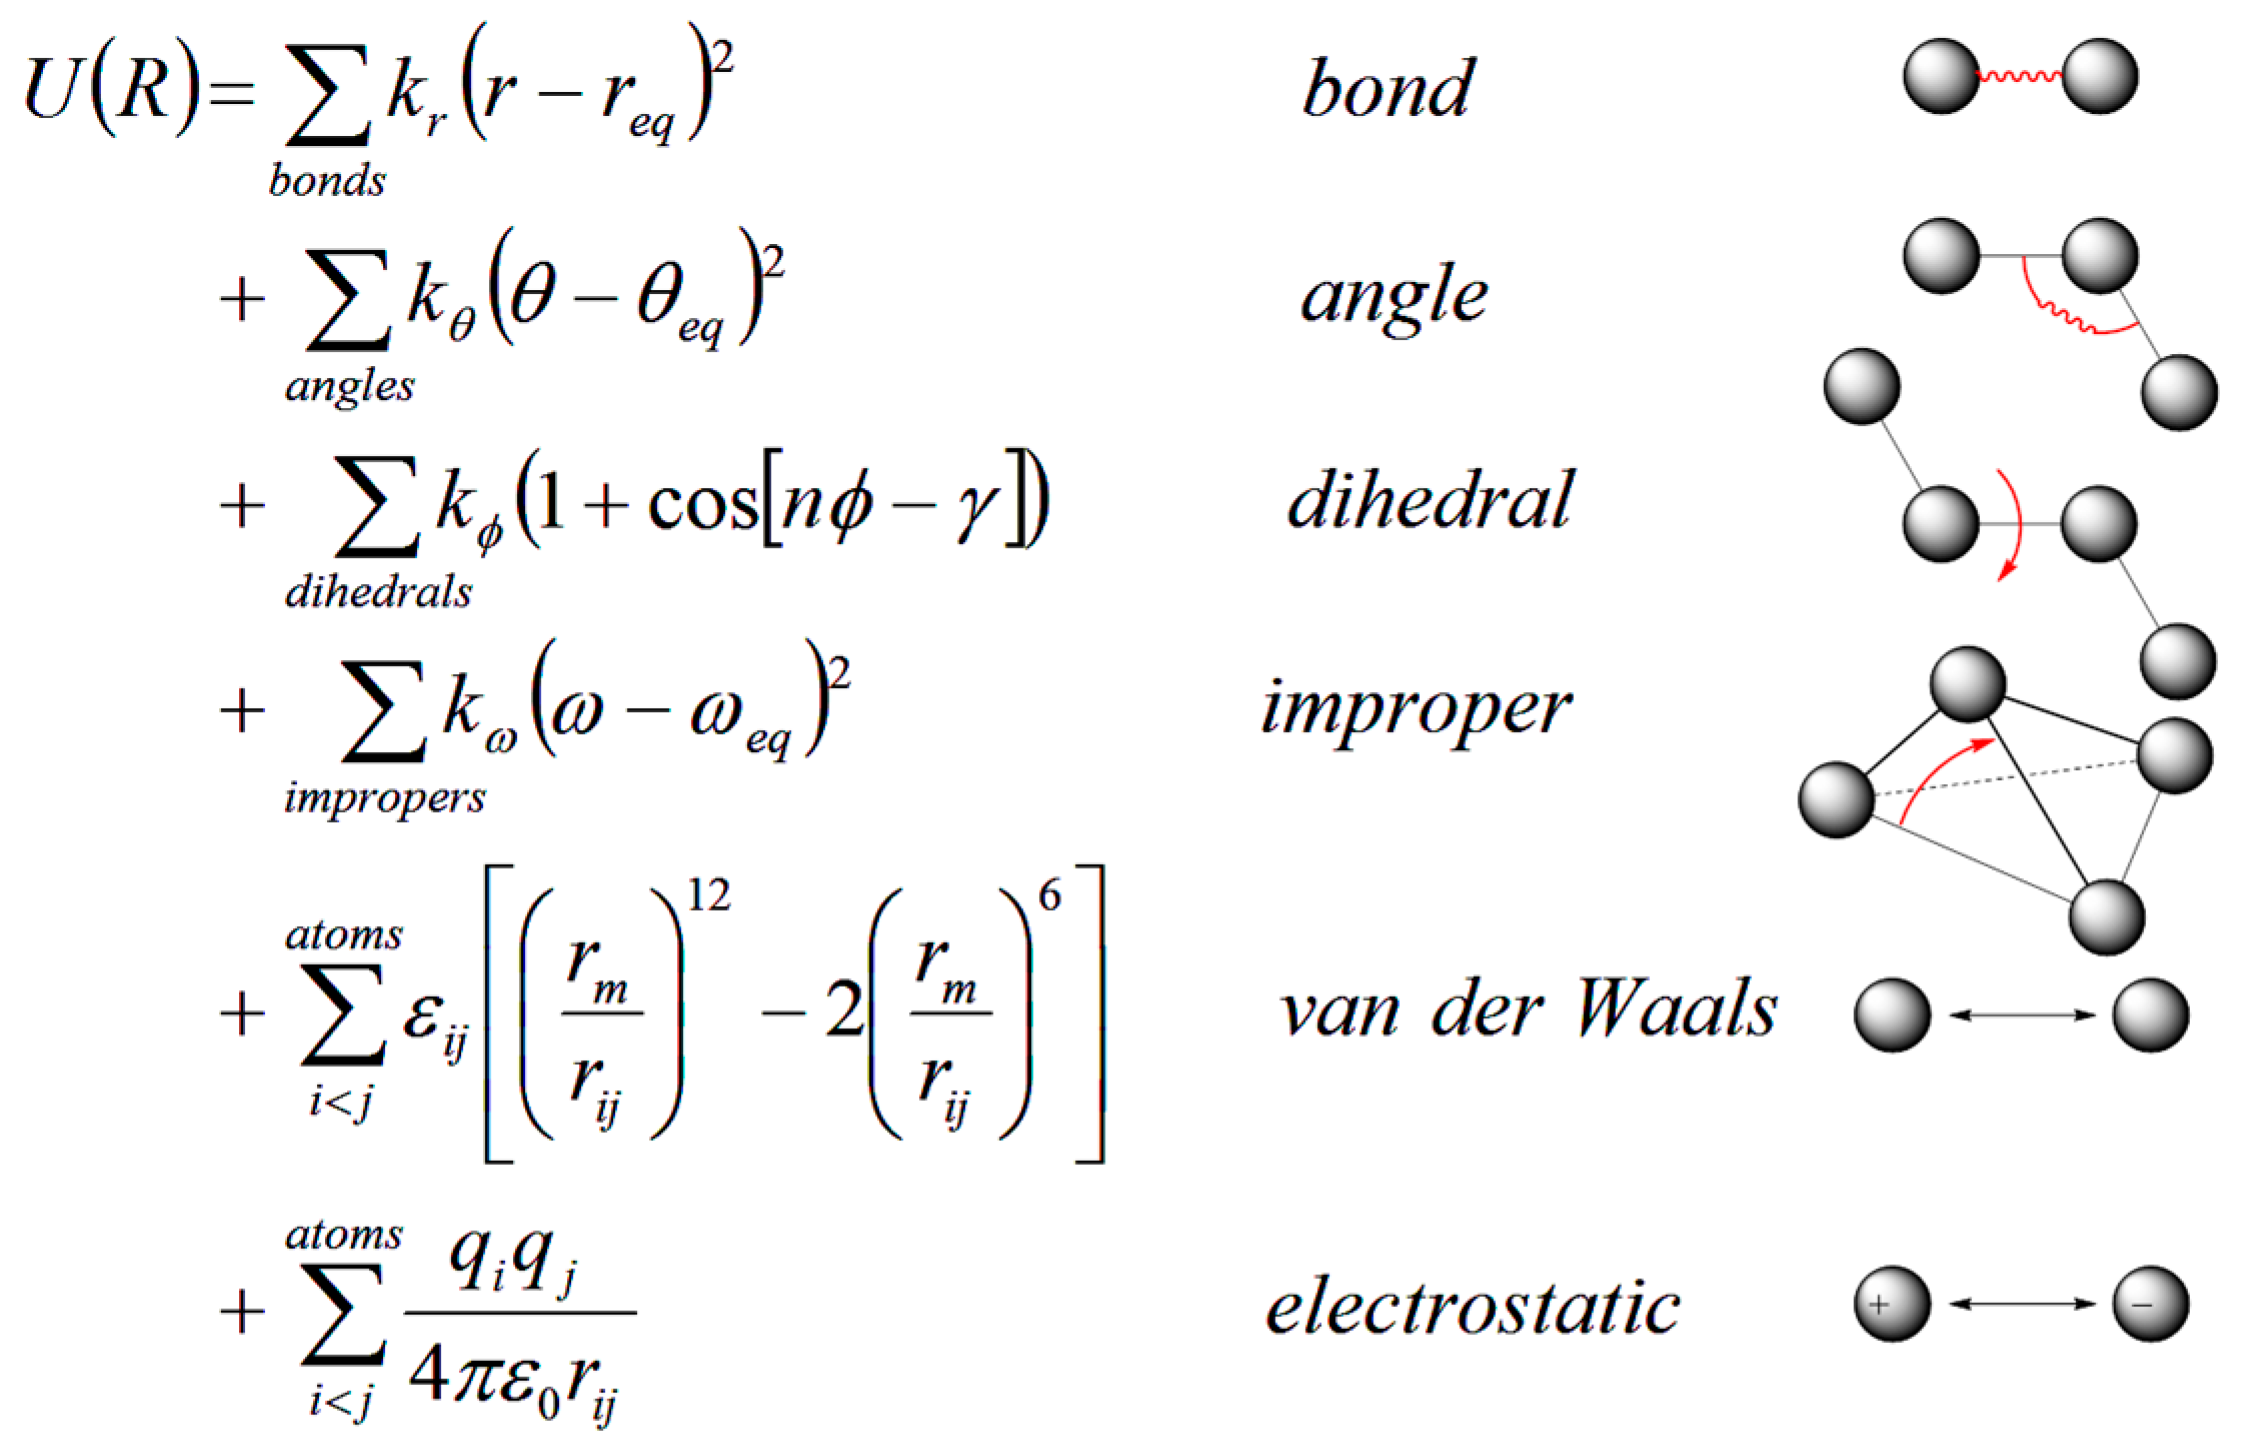
\includegraphics[width=1.0\linewidth]{img/ff.png} 
%	\caption{caption}
%	\label{fig:ff}    
%\end{figure}  
\newpage
By the level of functional description (number of terms) of the interactions in the force field, we distinguish force fields of three classes. Class 1 force fields contain the 5 terms mentioned in the two equations above (bond, angle, torsion, Lennard-Jones and electrostatic), examples of such FF are the DREIDING \cite{mayo_dreiding_1990}, AMBER \cite{brooks_charmm_2009}, GAFF \cite{wang_development_2004} and OPLS \cite{jorgensen_opls_1988}. In addition, class 2 force fields include bond-bond and bond-angle coupling terms, anharmonic terms simultaneously with all class 1 terms, examples of such fields are PCFF \cite{sun_ab_1994} or ReaxFF \cite{senftle_reaxff_2016}.  The third class includes fluctuations of charge distribution in time (charge polarization effect), and they are called polarizable FF. \cite{vanommeslaeghe_molecular_2014}

During the parameterization of force fields (FF), we start from the assumption of transferability,  similar chemical groups of different molecules interact in the same way. When constructing a force field for large molecules, we can use parameters obtained from data for small molecules, which are much more easily graspable and contain the same functional groups. \cite{monticelli_force_2013} In model development, our aim is to achieve the most universal description of the system while still closely corresponding to its actual state. This can be facilitated by employing higher-order terms; however, incorporating anharmonic and cross terms introduces the need for a greater amount of FF parameters. We strive to avoid situations where we employ an overly adapted and detailed model that merely reproduces inserted information without providing any predictive capabilities. \cite{vanommeslaeghe_molecular_2014}

According to the level of parameterization, there are 3 basic types of force fields. In the first case, where the parameters are determined for each individual atom in the system, including hydrogens, we speak of an all-atom force field. A united atom force field is one where we parameterize the individual functional groups (interaction centers), such an interaction center could be for example a methyl group. The third type of force field is coarse grained, used mainly for protein and polymer simulations, offering higher computational efficiency for long simulations of large molecules by grouping them into "superatoms". \cite{da_silva_are_2020}

\subsubsection{OPLS force field}

Optimized Potential for Liquid Simulations (OPLS) force field was developed by William L. Jorgensen \cite{jorgensen_opls_1988} at Purdue University and later at Yale University based on previously released Assisted Model Building and Energy Refinement (AMBER) force field developed by Peter Kollman's group. \cite{cornell_second_1995} The OPLS force field consists of following terms written in Equation \ref{eq:opls}. 
	
	\begin{equation}
		\begin{aligned}
			U_{\text{OPLS}} = & \sum_{\text{bonds}} \frac{1}{2} k_b(r-r_0)^2 + \sum_{\text{angles}} k_{\theta} (\theta-\theta_0)^2 \\
			& + \sum_{\text{torsions}} \Biggl( \frac {V_1} {2} \left [ 1 + \cos (\phi) \right ] + \frac {V_2} {2} \left [ 1 - \cos (2\phi) \right ] 
			+ \frac {V_3} {2} \left [ 1 + \cos (3\phi) \right ] + \frac {V_4} {2} \left [ 1 - \cos (4\phi) \right ] \Biggr) \\
			& + \sum_{i=1}^{N-1} \sum_{j=i+1}^N \left\lbrace 4\epsilon_{ij} \left[ \left( \frac{\sigma_{ij}}{r_{ij}} \right)^{12} - \left( \frac{\sigma_{ij}}{r_{ij}} \right)^6 \right] + \frac{q_iq_je^2}{r_{ij}} \right\rbrace f_{ij}
		\end{aligned}
		\label{eq:opls}
		\vspace{-0.4cm}
	\end{equation}
	
$i$ and $j$ denote different atom types, $N$ is the total number of atom pairs, $\epsilon_{ij}$, $\sigma_{ij}$ are LJ parameters, $r_{ij}$ is the distance between atoms $i$ and $j$, and $f_{ij}$ is scaling factor equals 0.5 for 1-4 interactions ($i,j$=1,4) and 1 otherwise.
	
\textbf{Bonds and angles} are described as harmonic oscillators in OPLS FF. The equilibrium parameters are obtained by structural methods, such as x-ray diffraction NMR experiments. The values for force constants are then fitted to experimental data taken from vibrational spectroscopy. In Figure \ref{fig:torsion} is the visualization of the constants.

Proper \textbf{dihedral angle} $\phi$ between atoms $i$, $j$, $k$, $l$ is represented in Figure \ref{fig:torsion}. The torsional energy is described as a cosine expansion, where the first term corresponds to the rotation periodic after 360$^\circ$, second term by 180$^\circ$, the third term by 120$^\circ$ and the fourth term by 90$^\circ$. Each of this term has a $V_n$ constant, representing the barrier for rotation along the proper dihedral angle, which is dependent both on the torsional energy and non-bonded forces. Different approaches could be chosen, one of them is obtaining the parameters by QM calculations. \cite{mackerell_empirical_2004} We first optimize the molecular geometry using QM methods and then we run scanning of dihedral angle of interest. At each step, we optimize geometry and calculate the change in potential energy.  Then we compute potential energy of each optimized geometry using MD with dihedral parameters set to zero. Then we can fit the parameters by subtracting the results of MD from QM, this corresponds exactly to the influence of dihedrals. To do this procedure first, all the other FF parameters should be known. 
\vspace{-0.2cm}
\begin{figure}[H]
	\centering
	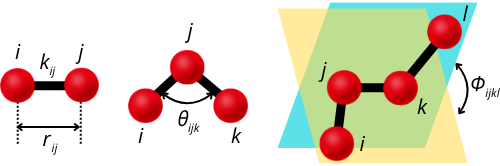
\includegraphics[width=0.60\linewidth]{img/uhly_canva.png} 
\vspace{-0.2cm}
\caption{Graphical representation of the terms from OPLS force field.}
\label{fig:torsion}  
\end{figure}
\vspace{-0.5cm}

\textbf{Charges} parametrization is also done by ab initio methods. When we are using the classical FF, the charges used to calculate the Coulomb potential remain the same during the simulations. Due to that, it is crucial to obtain the charges from an equilibrium state of the molecules in order to avoid any errors from having the charges taken from structures with higher energy. When obtaining the charges, the first step is to optimize the geometry using the appropriate level of theory. A commonly used method to achieve the charges is CHELPG (CHarges from ELectrostatic Potentials using a Grid based method) \cite{breneman_determining_1990}, based on adjusting the partial charges at the centers of the nuclei in order to get the best representation of the electrostatic potential given by the wave functions. Calculation of the charges are often done using quantum methods and basis sets such as B3LYP/cc-pVTZ or HF/6-31G**.

\textbf{Van der Waals} forces are most often represented by the Lennard-Jones (LJ) potential. The functional form with the illustration is in Figure \ref{fig:lj}. Lennard-Jones potential is a combination of two terms, repulsive term describes the Pauli repulsion at short distances and the attractive term describes the London dispersion force. The $\epsilon$ values are adjusted to experimental values of heats of vaporization and $\sigma$ parameters are adjusted to experimental densities and structural data. 

\begin{figure}[H]
	\centering
	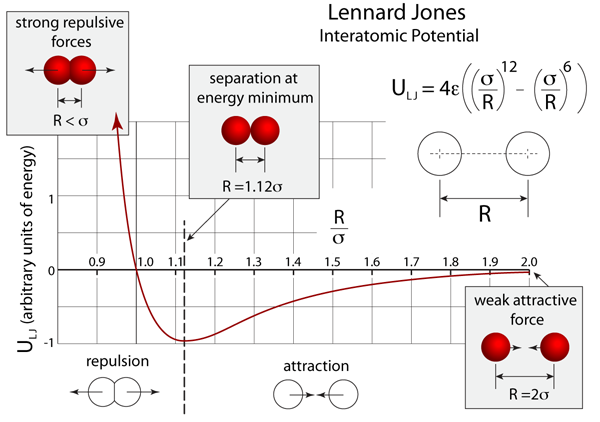
\includegraphics[width=1.0\linewidth]{img/lj.png} 
	\caption{Description of the Lennard-Jones potential taken from online source \cite{LJ}.}
	\label{fig:lj}    
\end{figure} 


\subsection{Periodic boundary conditions}
Due to the computational complexity, we are focused only on a small region of a very complex real system.  In order not to introduce errors caused by the boundaries of the system and interactions on them, we introduce periodic boundary conditions (PBC). This method is based on surrounding the simulated system with its periodic images, thus achieving an approximation by an infinite surface less system. We choose a shape of the simulation box that can be used to fill the space without problems, in our case a cubic box. For simulations in three dimensions, we usually introduce PBCs in the direction of all axes, which means that our simulated box is surrounded on all sides by a total of 26 replicas of the system. The behavior of the system is the same in all replicas, so we must include all the particles appearing in the replicas when calculating the pair interactions. \cite{allen_computer_2017}

\subsubsection{Setting the cutoff}
From the preceding paragraphs it is evident that the main problem in time complexity of the simulations is the evaluation of non-bonding energies. While the number of bonded terms increase linearly with the system size, the non-bonded terms show a quadratic increase in the number of contributions. A common strategy for reducing the computational time is to set specific cutoff distance, beyond which we neglect or estimate the non-bonded interaction energy contribution. We distinguish two types of interactions based on their decay with distance. First, the so-called short-range interactions decreasing faster than $1/r^3$ such as van der Waals ($1/r^6$) that could be neglected on a relatively short distance. By neglecting the van der Waals contributions at long distances, we introduce only a small numerical deviation for each pair, but the cumulative effect when all pairwise interactions are summed introduces larger deviations into the simulations. Theory says that van der Waals interactions are negligible beyond about 20 \AA, we choose 12 \AA~as the optimal cutoff in this work because of the optimal computational complexity. \cite{mdskripta}

For the long-range interactions, such as Coulombic interactions ($1/r$) the situation is not that easy and a larger cutoff than for van der Waals is required due to their long-range nature. The easiest option, as mentioned above, is to solve this issue by neglecting any contributions beyond the cutoff distance. The problem in that approach is that we introduce discontinuities in the potential and its derivatives. Better and more suitable approach, especially for periodic systems is called Ewald summation.


\subsubsection{Ewald summation}
The idea of Ewald summation is based on a mathematical trick where we divide a three-dimensional very slowly and only relatively converging infinite series into two series that converge much faster. In practice, this trick means surrounding each of the point charges with a shielding diffusion cloud of opposite charge, which shape is described by Gaussian function. This shadow cloud is then compensated by a charge of identical shape but opposite sign, illustration is in Figure \ref{fig:ewald}. Next, the contributions from the shadow cloud are summed in real space and the contributions of the compensation potential are summed in reciprocal space using the Fourier transform. Due to the smoothness of the charge distribution given by the Gaussian functions, this converges really fast in Fourier space. The width of the Gaussian peak determines the number of iterations to converge in reciprocal and direct space, the optimal width is then calculated in order to achieve even distribution of computational workload in both spaces. \cite{Sritterova}


\begin{figure}[htb!]
	\centering
	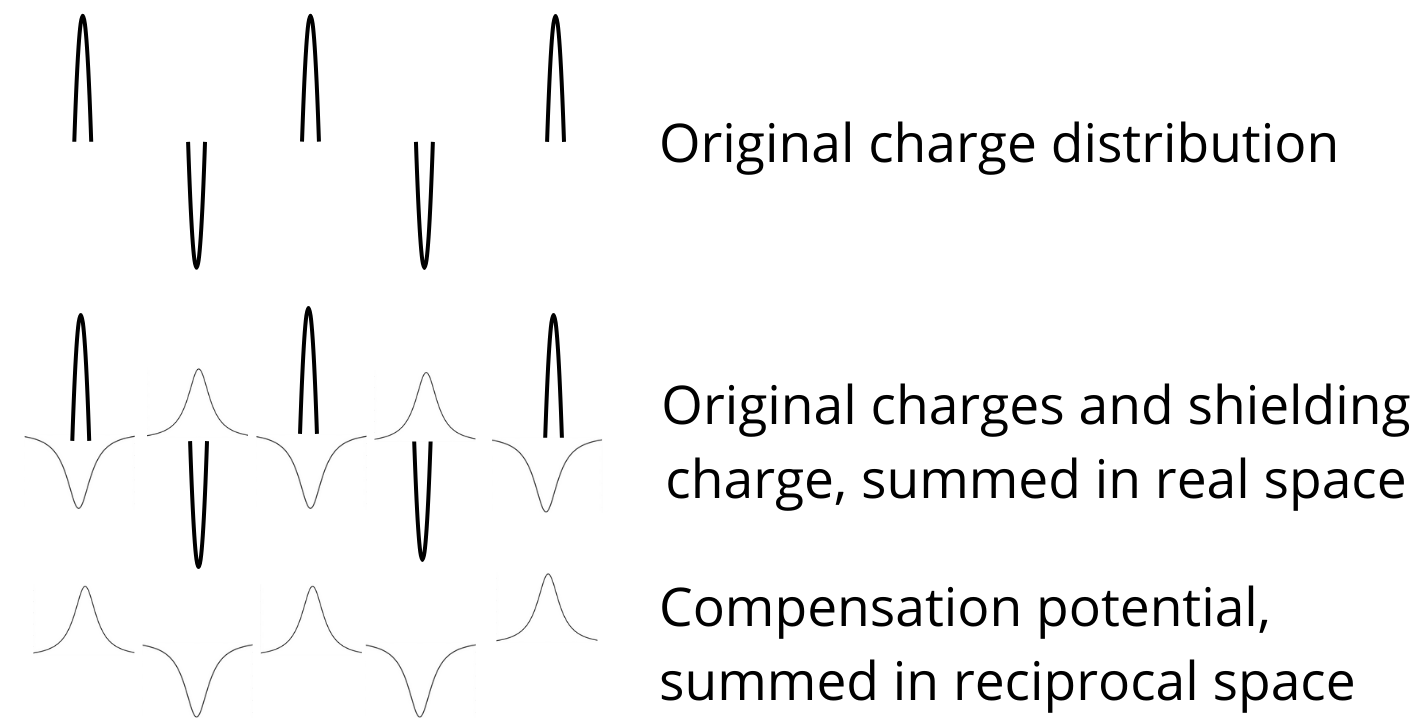
\includegraphics[width=0.8\linewidth]{img/ewald.png} 
	\caption{Illustration of the idea behind Ewald summation.}
	\label{fig:ewald}    
\end{figure} 

\subsubsection{Particle-Particle Particle-Mesh}
The Particle-Particle Particle-Mesh (PPPM) method \cite{eastwood_p3m3dpthree-dimensional_1980} is a development of the Ewald sum method. The PPPM method operates on the principle of decomposing the electrostatic potential into short-range and long-range components. The short-range interactions, which decay rapidly with distance, are typically calculated using direct methods like the Ewald summation or a cutoff-based approach. The long-range electrostatic potential is computed using a Fourier-based approach, where the charge distribution is mapped onto a grid using a fast Fourier transform (FFT). This grid-based representation allows for an efficient calculation of the potential at grid points using convolution techniques. \cite{Sritterova}


\subsection{Molecular dynamics}
The molecular dynamics method is based on solving the equations of motion of classical Newtonian mechanics for atoms. Let us choose the assumption that the interaction potential $U$ is continuous and differentiable. The force acting on the $i$ particle can thus be written as an equation \ref{sila1} 
\begin{equation}\label{sila1}
	f_i=-\frac{\partial U(r^N)}{\partial r_i}, \qquad i=1,...,N.
\end{equation}

In molecular dynamics, we are focused on the time development of the model. In other words, we are looking for the trajectory of the solution of the respective systems of differential equations. In Newtonian mechanics, acceleration is directly related to forces through the equations of motion. Formally, we can write the equation \ref{sila2}
\begin{equation}\label{sila2}
	\Ddot{r_i}=\frac{f_i}{m_i}, \qquad i=1,...,N,
\end{equation}
where the second time derivative of the positions appears on the left side. The equation \ref{sila2} is a system of 3$N$ ordinary differential equations for a set of $N$ atoms. As initial conditions, we usually choose the knowledge of all atomic positions $r_i$ and velocities $\dot{r_i}$ at the initial time $t=t_0$. 

We solve equation \ref{sila2} using the finite difference method when we track the desired solution in the form of the function $r_i(t), i=1,..,N$, in the time interval $[t_0,t_{max}]$ at discrete points of the form $t=t_0+kh$, where $h$ is the integration step and $k$ is a non-negative integer.

To find a solution, it is necessary to calculate the forces acting on individual particles at each step of the simulation. One of the methods that is applied in this area is the Verlet integration method. It is a simple and very effective method that provides sufficiently accurate results in the physico-chemical context. Its great advantage is the time-reversibility and the conservation of the total energy of the system~\cite{mdskripta}.

\subsubsection{Verlet integration}
Verlet integration method is a numerical method for integrating the equation \ref{sila1}. We express the second derivative using finite differences. From the second-order Taylor expansion $r_i(t\pm h)$ centred at $t$, we obtain the formula
\begin{equation}\label{sila3}
	\Ddot{r_i}=\frac{r_i(t-h)-2r_i(t)+r_i(t+h)}{h^2},
\end{equation}
binding atomic coordinates at three points in a time row ($t-h$, $t$ and $t+h$). We will use this relation to calculate $r_i(t+h)$. By substituting \ref{sila3} into \ref{sila1} we get 
\begin{equation}\label{sila4}
	r_i(t+h)=2r_i(t)-r_i(t-h)+h^2\frac{f_i(t)}{m_i}.
\end{equation}
In this formulation, we are able to calculate the new positions at time $t+h$ from knowledge of the forces at time $t$, the positions of the particles at time $t$ and the previous time $t-h$. The time reversibility of the method is clearly visible here. The advantage is that the force is calculated only once in each step of the simulation. For the position preceding the initial position ($t=-h$), we can use the expansion \ref{sila5}
\begin{equation}\label{sila5}
	r_i(-h)=r_i(t_0)-h\dot{r_i}(t_0)+h^2\frac{f_i(t_0)}{2m_i}.
\end{equation}

We can then calculate the position at $t=h$ from the known positions of $t=0$ and $t=-h$. There are not explicit velocities in the equations, algorithm with velocities often used by computation software is called Velocity Verlet algorithm. \cite{mdskripta}

\subsubsection{Constraint dynamics}

When integrating equations of motion, we often impose constraints on certain aspects of molecular geometries. The main reason is to enable using a longer simulation time step. If we simulate with a too large time step, we introduce large errors into the simulations, leading in extreme cases to a crash of the simulation. The calculated particle positions at time $t+h$ may lead to overlapping of particles, the calculated force acting on the particles may divert from physically reasonable configurations. Conversely, the use of inappropriately short simulation steps reduces the efficiency of the simulations (the most computationally and therefore time consuming element of the simulations is the calculation of the forces when integrating the equations of motion). \cite{mdskripta} The criterion determining the optimal step length is the accuracy of the conservation of total energy. The step length can be determined by an Nyquist-Shannon \cite{shannon_communication_1949} sampling theorem that says that the time step must be half or less of the period of the quickest dynamics exhibited in the system. Thus, for systems containing very light hydrogen atoms, we can either artificially increase the mass of the hydrogen atom while redistributing the masses of the other molecules to conserve the overall mass of the molecule, or fix the bond angles or bond lengths terminating in the hydrogen atoms. It is the fixation of hydrogen bond lengths that is most often implemented in the Verlet method, using an algorithm called SHAKE.  

\newpage
The SHAKE algorithm \cite{ryckaert_numerical_1977} is based on Verlet's integration method and is iterative. The first step is to initialize the initial velocities and positions of the atoms, then calculate the positions using Verlet's method without considering bond length constraint. We then create the $\lambda$ correction of the atom positions to constrain the bond length. Fixing the bond length allows us to use a longer time step (we are no longer limited by the motion of very light particles) and, unlike fixing angles, does not introduce large deviations in the simulations. \cite{mdskripta}

\subsection{Measuring the properties}
\subsubsection{Statistical ensembles}
MD gives us insight into the total energy of the system, which is naturally conserved in simulations. However, real systems are rarely thermodynamically isolated and we often expose the system to external pressure or heat exchange. Thus we speak of different statistical ensembles depending on the conservation of quantities.

As already mentioned, the natural ensemble is the so-called microcanonical ensemble, $\boldmath{NVE}$. Thermodynamically it is an adiabatically isolated and closed system, there is no heat exchange while maintaining the total number of particles, total energy and volume. 

Another commonly used ensemble is the canonical ensemble, often referred to as $\boldmath{NVT}$. Here, the system is maintained at constant temperature ($T$) and volume ($V$), allowing for heat exchange with a thermostat.

For many chemical systems, particularly those involving reactions in solution or under variable pressure conditions, the $\boldmath{NpT}$ ensemble is preferred. In this ensemble, both temperature and pressure are kept constant, ensuring that the system remains in equilibrium with its environment. The $NpT$ ensemble is valuable for studying systems where pressure effects play a significant role.


\subsubsection{Mean Square Displacement}
The Mean Square Displacement (MSD) is a measure of the average displacement of particles in a system over time, used to analyze the diffusive behavior of particles. The average squared distance traveled by particle is measured, Equation \ref{eq:MSD}

\begin{equation}\label{eq:MSD}
MSD(t) = \frac{1}{N} \sum_{i=1}^{N} \left\langle \left| \mathbf{r}_i(t) - \mathbf{r}_i(0) \right|^2 \right\rangle,
\end{equation}

where $\mathbf{r}_i(0)$ is the initial position and $\mathbf{r}_i(t)$ is the particle position at time $t$. We can obtain diffusion coefficient by applying the following Equation \ref{eq:Di} \cite{braun_best_2019}. 

\begin{equation}\label{eq:Di}
	D = \frac{\text{MSD}(t)}{2dt}
\end{equation}

where $d$ is the dimensionality of the track, $d$=3 in three dimensions.

\subsubsection{Radial Distribution Function}
When we are studying the contacts in liquids, the basic structural quantity is radial distribution function (RDF). As distribution function, it describes the probability of finding a particle at distance $r$ of some other particle. \cite{mdskripta} 

When we want to extract the RDF from MD simulations, the following strategy is applied. First we have to choose the particle, which surrounding we want to study. Then the space around this particle is divided into concentric spherical shells each having a specific radius. The number of particles inside each shell is counted and the histogram created is then normalized by the volume of each shell and total number of particles. For uncorrelated particles, ideal gas or liquid particles at long distances, the RDF is equal to one. 

The first peak of RDF corresponds to the nearest neighbors of the particle. The position on $x$-axis is determined by the contact distance. The following minima correspond to the steric shielding of the first neighbours. The second peak has the meaning of the second shell of neighbors and so on for later peaks. The amplitude of the peaks corresponds to the relative occurrence in the mixture, the more contacts in the bulk mixture, the probability (height of the peak) is higher. \cite{mdskripta}

When we want to extract more information from RDF and study how many particles are on average to the specific distance, we are talking about the cumulative RDF (CRDF). The CRDF is a function of coordination number depending on distance, that we can obtain by integrating the RDF from 0 to a desired distance, usually to the first neighbor cutoff, which is given by the RDF minimum. The integration is shown in Equation \ref{eq:CRDF}, where $g(r)$ is the RDF. The number of particles within the radius $r$ is then CRDF multiplied by density.~\cite{mdskripta}

\begin{equation}\label{eq:CRDF}
	\text{CRDF}(r) = \int_{0}^{r} 4\pi r'^2 g(r') \, dr'
\end{equation}

\subsubsection{Block averaging scheme}
When we are extracting the properties such as volume, density or energy, we are handling with average values obtained from MD simulation. MD simulation data often exhibit correlations between consecutive frames due to the deterministic nature of the molecular dynamics algorithm. When we are estimating the uncertainties or errors associated with calculated properties, we have to consider that the simulated data might be correlated and use appropriate statistical methods. 

The often used method to evaluate the standard errors is the block averaging scheme. The trajectory data generated from the MD simulation are divided into non-overlapping blocks of equal length. We are assuming, that data within those blocks are no more correlated. For each block, the average value of the property and its standard deviation is calculated from the simulation data. Finally, the averages and standard deviations from all blocks are combined to obtain an overall estimate of the uncertainty in the property of interest. The algorithm used in this work is described more into details by Allen.  \cite{allen_computer_2017}


